\documentclass[tikz]{standalone}
\usepackage{tikz}

\begin{document}
  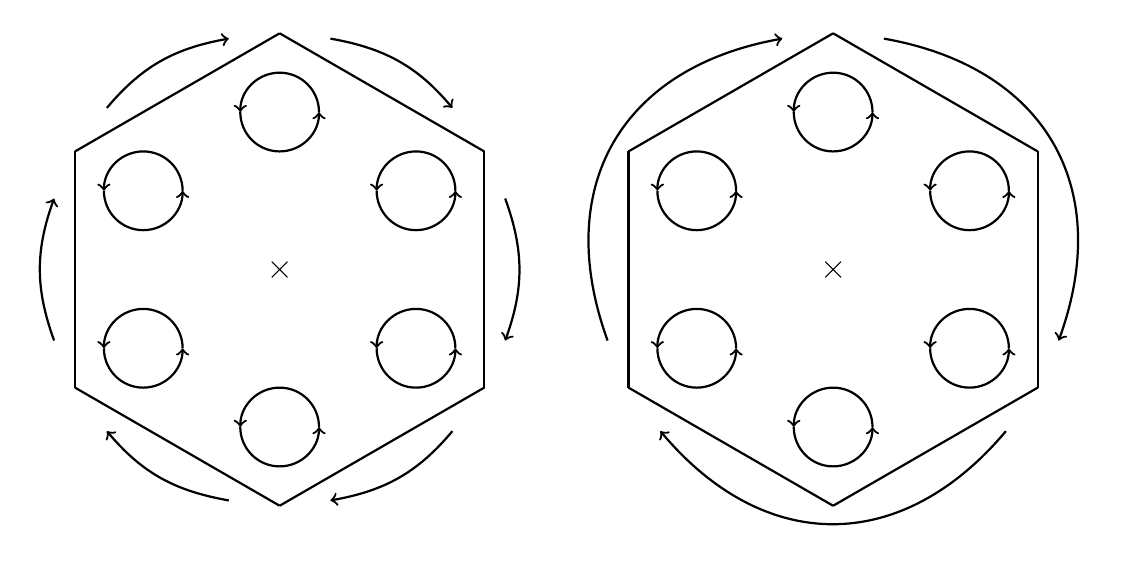
\begin{tikzpicture}
    \draw % x marks the spot!
      (-0.1,-0.1)--(0.1,0.1)
      (-0.1,0.1)--(0.1,-0.1)
    ;
    \path (-3.2,0)--(3.2,0); % Set left/right padding
    \foreach \t in {30,90,...,330} {
      \node (A\t) at ({3*cos(\t+10)},{3*sin(\t+10)}) {};
      \node (B\t) at ({3*cos(\t+50)},{3*sin(\t+50)}) {};
      \draw[thick, ->] (B\t) to[out=\t-40, in=\t+100] (A\t);
      \draw[thick] ({3*cos(\t)},{3*sin(\t)}) -- ({3*cos(\t + 60)},{3*sin(\t + 60)});
      \foreach \th in {0, 180} {
        \draw[thick, ->] ({2*cos(\t)+cos(\th)*0.5},{2*sin(\t)+sin(\th)*0.5}) arc (\th:\th+180:0.5);
      }
    }

  \draw[xshift=20em] % x marks the spot!
    (-0.1,-0.1)--(0.1,0.1)
    (-0.1,0.1)--(0.1,-0.1)
  ;
  \path[xshift=20em] (-3.2,0)--(3.2,0); % Set left/right padding
  \foreach \t in {30,90,...,330} {
    \node[xshift=20em] (A\t) at ({3*cos(\t+10)},{3*sin(\t+10)}) {};
    \node[xshift=20em] (B\t) at ({3*cos(\t+50)},{3*sin(\t+50)}) {};
    \draw[xshift=20em, thick] ({3*cos(\t)},{3*sin(\t)}) -- ({3*cos(\t + 60)},{3*sin(\t + 60)});
    \foreach \th in {0, 180} {
      \draw[xshift=20em, thick, ->] ({2*cos(\t)+cos(\th)*0.5},{2*sin(\t)+sin(\th)*0.5}) arc (\th:\th+180:0.5);
    }
  }

  % \foreach \t in {30,150,270} {
    \draw[xshift=20em, thick, ->] (B150) to[out=150-40, in=90+100, looseness=1.2] (A90);
    \draw[xshift=20em, thick, ->] (B270) to[out=270-40, in=210+100, looseness=1.2] (A210);
    \draw[xshift=20em, thick, ->] (B30) to[out=30-40, in=330+100, looseness=1.2] (A330);
  % }

  \end{tikzpicture}
\end{document}
